\section{Integrationstest}
Integrationstests udføres for at checke om diverse moduler virker sammen. Helt konkret drejer det sig om at finde de komponenter der forårsager \textit{intercomponent failures}. De fleste \textit{interoperability} fejl findes ikke med \textit{component scope testing} Det er vigtigt at teste dette før der testes i \textit{system scope}.\\

Måden hvorpå en integrationstest adskiller sig fra en unittest er ved at den ikke er konsistent og/eller har en eller flere \textit{rigtige} afhængigheder. En test der f.eks. afhænger af \textit{DateTime}, er ikke længere konsistent idet tiden ændrer sig for hver test.

\subsection{Forarbejde og strategi}

Før man begynder at integrationsteste er der nogle ting som bør være opfyldt:

\begin{itemize}
	\item Unittests skal være færdige. Dette gælder for samtlige metoder.
	\item Systemets dependancy tree skal være kendt!
	\item Hvilke komponenter er i fokus?
	\item I hvilken rækkefølge skal komponenterne testes?
\end{itemize}

\subsubsection{Dependancy trees}
Dependancy trees er en måde at visualisere afhængighederne i et projekt. Arve-heirakiet vises ikke. Det er vigtigt at have et overblik over sine dependancies når man skal planlægge integrationstest. På figur~\ref{fig:dependancyATM} vises et uddrag fra ATM opgavens dependancy tree.

\begin{figure}[H]
	\centering
	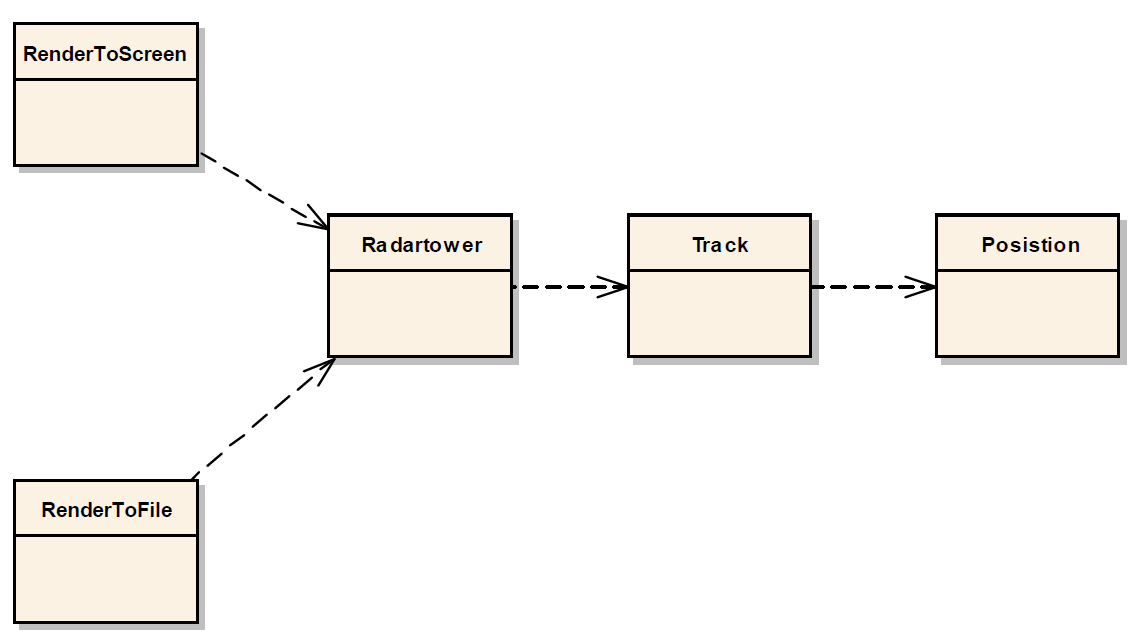
\includegraphics[width=0.78\linewidth]{figs/dependancyATM.PNG}
	\caption{Uddrag fra ATM's dependancy model. Venstre side er toppen af træet.}
	\label{fig:dependancyATM}
\end{figure}

Dependancy træet er opbygget så høj niveau modulerne ligger i den ene ende og lav niveau modulerne i den anden ende.

\subsubsection{Drivers}

Sæt at vi har to komponenter: A og B, som vist i figur~\ref{fig:driver}. Hvis A er færdig og skal testes, laver vi en stub for B. 
Omvendt hvis B er færdig og A mangler, vil vi lave en \textit{driver} for A, som kan simulere et kald på B.

Et eksempel på en driver i unittests kan være vores \textit{TextFixture} klasse, som laver kaldene på \textit{\_uut} under test.

\begin{figure}[H]
\centering
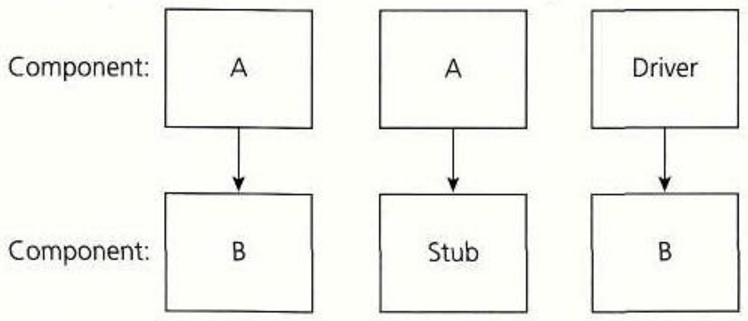
\includegraphics[width=0.6\linewidth]{figs/driver}
\caption{UML for driver og stubbe.}
\label{fig:driver}
\end{figure}

\subsection{Typer af integrationstest}
Der findes flere måder at integrationsteste på.

%%%%%%%%%%%%%%%%%%%%%%%%%%%%%%%%%%%%%%%%%%%%%%%%%%%%%%%%%%%%%%%%%%%%%%%%%%%%%%%%%%%%%%%%%%%%%%%%%%

\subsubsection{Big Bang testing}
I en \textit{Big Bang} integrationstest, sammensættes alle komponenter, så det komplette system dannes. Herefter testes systemet.

\paragraph{Fordele}
\begin{itemize}
	\item Man slipper for at planlægge sin test
	\item Nemt at bruge i mindre systemer
\end{itemize}

\paragraph{Ulemper}
Der er en del ulemper ved denne integratoinstest model.

\begin{itemize}
	\item Man finder først fejlene når alle komponenter sættes sammen.
	\item Svært at isolere de fundne fejl.
	\item Stor sansynlighed for at misse kritiske fejl, som senere kan vise sig.
	\item Svært at dække alle test scenarier uden at misse enkelte.
	\item Bug-fixing er last-minute og er derfor ofte af dårlig kvalitet.
\end{itemize}

%%%%%%%%%%%%%%%%%%%%%%%%%%%%%%%%%%%%%%%%%%%%%%%%%%%%%%%%%%%%%%%%%%%%%%%%%%%%%%%%%%%%%%%%%%%%%%%%%%

\subsubsection{Bottom-Up testing}
Starter i bunden af dependancy træet - nederste lag testes først.

\paragraph{Fordele}

\begin{itemize}
	\item Ingen eller få stubbe, da vi skal ikke fake dependancies.
\end{itemize}

\paragraph{Ulemper}

\begin{itemize}
	\item Kræver mange drivere.
	\item Udsætter test af kritiske kontrol interfaces (komponenter højere oppe i træet).
\end{itemize}

\begin{figure}[H]
	\centering
	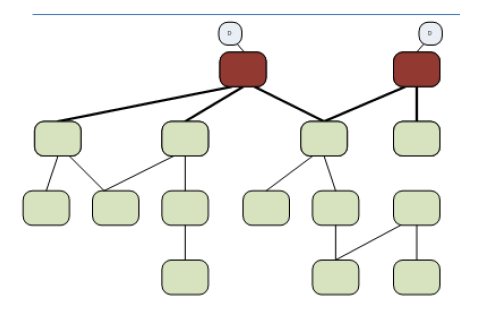
\includegraphics[width=0.5\linewidth]{figs/bottomUp.PNG}
	\caption{Illustration af Bottom-Up testing.}
	\label{fig:bottomUp}
\end{figure}

%%%%%%%%%%%%%%%%%%%%%%%%%%%%%%%%%%%%%%%%%%%%%%%%%%%%%%%%%%%%%%%%%%%%%%%%%%%%%%%%%%%%%%%%%%%%%%%%%%

\subsubsection{Top-Down testing}
Starter i toppen af dependancy træet - øverste lag testes først.

\paragraph{Fordele}

\begin{itemize}
	\item Få drivere.
	\item Mange stubbe, hvilket er OK med et isolation framework.
	\item Man udsætter ikke testing af kontrol komponenter.
	\item God til at arbejde samtidigt på HW og SW.
\end{itemize}

\paragraph{Ulemper}

\begin{itemize}
	\item Bruger mange stubbe. Et isolation framework gør det dog lettere.
	\item Svært at repræsentere low-level interfaces i toppen. 
\end{itemize}

\begin{figure}[H]
	\centering
	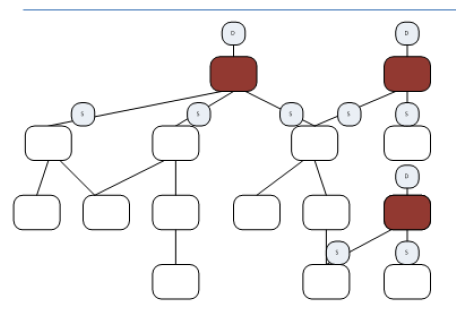
\includegraphics[width=0.5\linewidth]{figs/topDown.PNG}
	\caption{Illustration af Top-Down testing.}
	\label{fig:topDown}
\end{figure}

%%%%%%%%%%%%%%%%%%%%%%%%%%%%%%%%%%%%%%%%%%%%%%%%%%%%%%%%%%%%%%%%%%%%%%%%%%%%%%%%%%%%%%%%%%%%%%%%%%

\subsubsection{Collaboration testing}
Der vælges en 'vej' gennem dependancy træet, fra top til bund. Eksempelvis en \textit{User Story} eller \textit{Use Case}. I collaboration test tager man en "gren" af gangen i dependency træet.

\paragraph{Fordele}

\begin{itemize}
	\item Intuitivt - Kan følge use cases/user stories.
	\item Specielt brugbart for et højniveau system scope test.
\end{itemize}

\paragraph{Ulemper}

\begin{itemize}
	\item Testede sub-components testes ikke enkeltvis.
\end{itemize}

\begin{figure}[H]
	\centering
	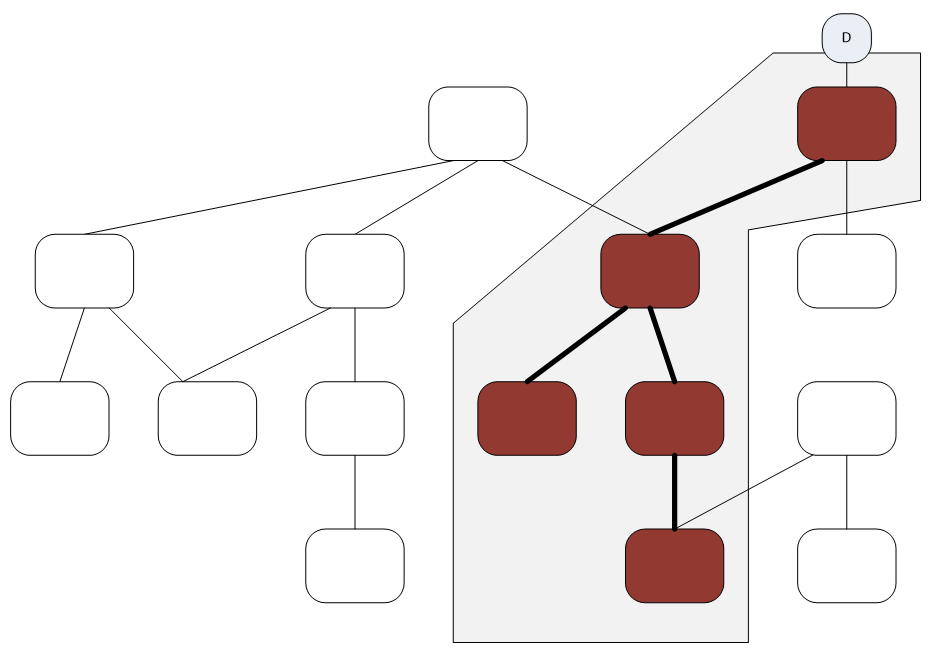
\includegraphics[width=0.5\linewidth]{figs/collaborationTesting.PNG}
	\caption{Illustration af Collaboration testing.}
	\label{fig:collaborationTesting}
\end{figure}

%%%%%%%%%%%%%%%%%%%%%%%%%%%%%%%%%%%%%%%%%%%%%%%%%%%%%%%%%%%%%%%%%%%%%%%%%%%%%%%%%%%%%%%%%%%%%%%%%%

\subsubsection{Sandwich testing}
Top-down og Bottom-up kombineres.

\paragraph{Fordele}

\begin{itemize}
	\item Man kan bruge både Bottom-Top og Top-Down hvis det giver mening.
	\item Mange af ulemperne ved Bottom-Top og Top-Down fjernes.
	
	\begin{itemize}
		\item Fordelen ved Buttom-Up er at bugs er lettere at finde.
		\item Ved Top-Down er det nemmere at finde manglede forbindelser mellem komponenter.
	\end{itemize}
	
\end{itemize}

\paragraph{Ulemper}

\begin{itemize}
	\item Kræver en stor del planlægning.
	\item Kan ikke anvendes på små systemer.
\end{itemize}

\begin{figure}[H]
	\centering
	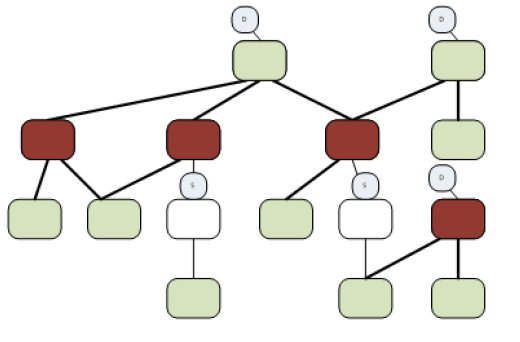
\includegraphics[width=0.5\linewidth]{figs/sandwich.PNG}
	\caption{Illustration af Sandwich testing.}
	\label{fig:sandwich}
\end{figure}






























